\begin{minipage}{0.49\linewidth}
    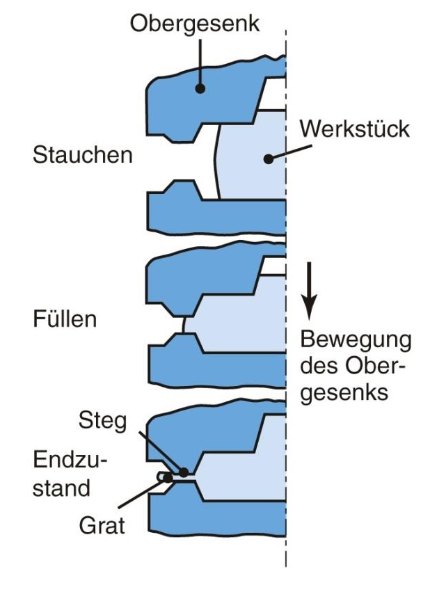
\includegraphics[width = 30mm]{src/images/Gesenkschmieden.png}
\end{minipage}
\begin{minipage}{0.49\linewidth}
    \textbf{Verfahren:}\\
    Umformen in geschlossenem Werkzeug (Gesenk).\\
    Bei sicherheitsrelevanten Teilen (Zahnräder, Pleuel, Getriebeteile). \\
    
    \textbf{Besonderheiten:}\\
    Erzeugt einen günstigen Faserverlauf (reduzierte Rissempfindlichkeit).\\
    Verschleissbelastung der Form sehr hoch.\\
    
\end{minipage}
